% ****** Start of file apssamp.tex ******
%
%   This file is part of the APS files in the REVTeX 4.1 distribution.
%   Version 4.1r of REVTeX, August 2010
%
%   Copyright (c) 2009, 2010 The American Physical Society.
%
%   See the REVTeX 4 README file for restrictions and more information.
%
% TeX'ing this file requires that you have AMS-LaTeX 2.0 installed
% as well as the rest of the prerequisites for REVTeX 4.1
%
% See the REVTeX 4 README file
% It also requires running BibTeX. The commands are as follows:
%
%  1)  latex apssamp.tex
%  2)  bibtex apssamp
%  3)  latex apssamp.tex
%  4)  latex apssamp.tex
%
\documentclass[%
reprint,
superscriptaddress,
citeautoscript,
%groupedaddress,
%unsortedaddress,
%runinaddress,
%frontmatterverbose, 
%preprint,
%showpacs,preprintnumbers,
%nofootinbib,
%nobibnotes,
%bibnotes,
 amsmath,amssymb,
 aps,
 prl,
%pra,
%prb,
%rmp,
%prstab,
%prstper,
floatfix,
]{revtex4-1}

\usepackage{graphicx}% Include figure files
\usepackage{dcolumn}% Align table columns on decimal point
\usepackage{bm}% bold math
\usepackage{color,soul} % highlight text
%\usepackage{hyperref}% add hypertext capabilities
%\usepackage[mathlines]{lineno}% Enable numbering of text and display math
%\linenumbers\relax % Commence numbering lines

%\usepackage[showframe,%Uncomment any one of the following lines to test 
%%scale=0.7, marginratio={1:1, 2:3}, ignoreall,% default settings
%%text={7in,10in},centering,
%%margin=1.5in,
%%total={6.5in,8.75in}, top=1.2in, left=0.9in, includefoot,
%%height=10in,a5paper,hmargin={3cm,0.8in},
%]{geometry}

\begin{document}


\preprint{APS/123-QED}

% \title{Predicting band gap correction for perovskite oxide using high throughput and machine learning}
\title{Searching for Hidden Trend of Perovskite Materials Band Gaps}
% Force line breaks with \\
%\thanks{A footnote to the article title}%

\author{Wei Li}
\affiliation{Department of Materials Science and Engineering, University of Delaware, Newark, DE 19716, USA}
\author{Zigeng Wang}
\affiliation{Computer Science and Engineering Department, University of Connecticut, USA,19716, USA}
\author{Xia Xiao}
\affiliation{Computer Science and Engineering Department, University of Connecticut, USA,19716, USA}
\author{Zhiqiang Zhang}
\affiliation{Department of Physics, University of Delaware, Newark, DE 19716, USA}
\author{Rajasekaran, Sanguthevar}
\affiliation{Computer Science and Engineering Department, University of Connecticut, USA,19716, USA}
\author{Bharat Medasani}
\affiliation{Delaware Energy Institute, University of Delaware, Newark, DE 19702, USA}
\author{Anderson Janotti}
\affiliation{Department of Materials Science and Engineering, University of Delaware, Newark, DE 19716, USA}
\email{janotti@udel.edu}

\date{\today}% It is always \today, today,
             %  but any date may be explicitly specified
\begin{abstract}

Machine learning has been recently used for novel perovskite designs owing to the availability of a large amount of applications because of the structure flexibility with multiple A-B-X combination. A tremendous amount of potential element combinations can be considered within perovskite structures, suggesting that there should still be hidden and undiscovered perovskite materials useful for solar light capturing. However, trustworthy results should be based on the valid and reliable data that can reveal the nature of materials as much as possible. We carefully generated the HSE and PBEsol datasets and it indicate that the valence band maximum (VBM) decreased 1 eV and conduction band minimum (CBM) increased 0.5 eV. We used machine learning with a multiple models approach accurately predict the HSE06 VBM, CBM and E$_{g}$ correction with accuracy of -0.145 eV, by quantitatively analyzing the valence band maximum (VBM) and conduction band minimum (CBM) offset. Not only does this resulting tool provide the ability to accurately predict the HSE06 band gap based on the PBEsol results but also the speed of the prediction based only on the cubic structure will make this a great resource to screen functional pervoskite materials. And this design represents a powerful database and tool paves a way for mapping the vast materials landscape and accelerating discovery. 


%\begin{description}
%\item[Key words]
%Secondary publications and information retrieval purposes.
%\end{description}
\end{abstract}

%\pacs{Valid PACS appear here}% PACS, the Physics and Astronomy
                             % Classification Scheme.
%\keywords{Suggested keywords}%Use showkeys class option if keyword
                              %display desired
\maketitle

%\tableofcontents

\section{Introduction}
 
 \begin{figure}[ht]
\begin{center}
\includegraphics[width=2.6 in]{Figures/Fig1.eps}
\end{center}
\caption{ Crystal structures of garnet and perovskite prototypes.Green, blue and red spheres are atoms of A, B and O sites, respectively. a crystal structrure of $Pm\bar{3}m$ cubic structure. b crystal structure of $I4_mmm$ tetragonal structure. c crystal structure of $Pnma$ orthohombic structure. d crystal structure of $R\bar{3}c$ Rhombohedral 
}
\label{fig1}
\end{figure}

Density functional theory (DFT)\cite{Kohn1964,Kohn1965}  is often used to predict crystal structure lattice parameters, within 1-2\% of the experimental values and the scalability of computations makes it possible to make predictions on thousands of materials.  However, there is a systematic under-estimation of the band gap, E$_g$, compared with the experimental values when employing standard exchange and correlation functionals such as the generalized gradient approximation as proposed by Perdew, Burke, and Ernzerhof (PBE).  Hybrid functionals  \cite{Heyd2003,Heyd2006} or the Green’s function quasi-particle GW methods \cite{Luoie1996,Kresse2006} improve accuracy, yet are much more expensive computationally, precluding their systematic use in searching over thousands of compounds. To accelerate the discovery and development of new functional materials, it is desirable to have an automating and scaling computational approach that predicts accurate values for band gaps at the speed or faster than DFT-PBE calculations. 

Over the last decade, ML has been applied to materials science problems in a variety of directions, such as prediction and classification of crystal structures\cite{Fischer2006,CARR2009339,Pilania2015,Yamashita2018} , development of interatomic potentials \cite{Hobday1999,Handley2010,Schneider2017} finding of optimal density functionals for density functional theory \cite{Wellendorff2012,Snyder2012,Brockherde2017,Pilania2013}, and building of predictive models of material properties\cite{Pilania2013,Lee2016,Pilania2016,Bart2017}. Instead of the conventional computational materials design, which derived materials properties according to physical law, for example, solving the Kohn-Sham equation, ML can learn the hidden rules based on a large data set and build a model to make corresponding predictions. 

% The statistical learning has emerged as a promising tool for predicting the cohesive energy, lattice thermal conductivity, band gaps, free energy, and heat capacity within reasonable time.


\begin{figure*}[ht]
\begin{center}
\includegraphics[width=6.0in]{Figures/fig2_v1.eps}
\end{center}
\caption{ (b) The HSE06 functional correction comparing with PBEsol functional for the band gap (light green), VBM offset(lightblue) and CBM offset(darkred). (b) schematic demonstration of the band edge offset for ABO$_{3}$. 
}
\label{fig2}
\end{figure*}

Perovskite materials have garnered much attention due to having ideal band gaps for capturing solar light, leading to the design of photovoltaic systems \cite{Pilania2013,Lee2012}. A tremendous amount of potential element combinations can be considered within perovskite structures, suggesting that there should still be hidden and undiscovered perovskite materials useful for solar light capturing. So far, the main data for perovskite formability can be found in a few articles that summarized the existing experimental data and prevalent databases. High throughput first principle calculations have previously been used to screen for potential perovskite materials for solar light capturing\cite{Huo2018, Sun2015}, but such calculations are found to leave unexplored spaces of perovskite materials due to the limitation of heavy computational times. 

% This will enable us to provide high fidelity band gaps without a significant increase in computational cost.

% Machine learning and deep learning models are implemented in this project in order to uncover hidden trends and link to the PBE and HSE06 functional band gap of the perovskite materials. And it is able to reveal the descriptors determining the band gap within perovskite materials data, then rapid prediction of perovskite materials. 

In this project we developed a machine learning models for mapping DFT-PBE computed band gaps of perovskites into HSE06 band gaps, which agrees very well with experimental results. To generate DFT based observables and reliable database, we are calculating DFT bandgaps via high-throughput approach and find out the band gap correction and band offset between two approximations. 
% A data set comprising 383 perovskite was generated by performing the full DFT relaxation and energy calculations on all allowed species on the A, B sites. 
Machine learning models are implemented in this project in order to uncover hidden trends and link to the PBE and HSE06 functional band gap of the perovskite materials. And it reveals the descriptors determining the band gap within perovskite materials data with accuracy of 0.145 eV. Later on, we plan to extend this approach to explore the electronic structure of chalcogenides, and halides. 

% Thus, trends and periodicities hidden within the data of 19000 perovskite materials are sought after and hidden perovskite materials for applications in capturing solar light are explored through the use of materials informatics.
% Several research groups have demonstrated the benefits of automating and scaling computational property. For example, an overview of high-throughput band structure calculations by Curtarolo et al. [6] New materials for radiation detectors is suggested by screening about 22,000 materials by Hachmann, et al. [7]

% If the machine is able to determine the relation between data trends
% and properties, one can then consider it possible to design
% materials directly from the desired materials properties.5


% Perovskite materials have garnered much attention due to having ideal band gaps for capturing solar light, leading to the design of photovoltaic systems 9−12 A tremendous amount of potential element combinations can be considered within perovskite structures, suggesting that there should still be hidden and undiscovered perovskite materials useful for solar light capturing.


\section{Method and computational details}
% Our project is designed to develop a database of calculated band gaps, starting with perovskite class of materials. 

% It is therefore of high technological interest to explore all possible perovskite materials with desirable electronic properties for optoelectronic applications.   
First-printciples calculations based on DFT are carried out based on the Vienna ab initio simulation packaged with plane-wave pseudopotential method\cite{}. The wave functions are expaned in the plane wave up to a cutoff energy of 650 eV. The exchange-correlation function we used in the general approximation of Perdew, Burke and Drnzernhof. A 9$\times$ 7$\times$ 9, 7$\times$ 15$\times$ 5, and 9$\times$ 9$\times$ 11 k-point grid was used in the PBEsol calculations for the case of cubic, tetragonal and orthorhombic structure optimization and electronic structure calculations. Hybrid functional at HSE06 level has been used
to accurately determine the band gap. 
 
The machine learning model is developed for the given band gap data set {X, y}, which maps input feature set X to the targeted HSE band gap y. Here, X = ${x_{i}}_{i = 1} ^{n}$ consists of $n$ individual features (with $n$ = 4). These relevant features are selected by the regression technique ( XGBoost ) and reduced to in the feature set. To build the learnign model, {X, y} is split into the training, testing and validation sets in the ratio of 80:15:5. 

\section{Results and Discussions}

% For each compound, four common phases, as shown inFig.~\ref{fig1}, are considered. Those four space groups dominate the crystal structure of existing oxides $ABO_{3}$ compounds. Cubic phase is the ideal perovskite structure without distortion, as shown in Fig.1(a). By considering 118 compounds with four crystal phase, we have a total of 590 systems of interest for further study.
% . With octahedral rotation and different phase, approximately 1000 materials will be used in our analyze at the beginning, and it will involve more materials later on.


% This dataset was randomly divided into training, validation and test data in the ration of (7:2:1). We find that this architecture yields a small root mean square error(RMSE) of ? eV, as well as the smallest standard deviation ... For comparison, the error in the DFT Eg of perovskite relative to experimental values is around ? eV.   

The systematic underestimation of DFT with standard exchange and correlation functional such as LDA or PBE/PBEsol stems from the well-known discontinuity in the derivative of exchange and correlation functional as the number of electrons deviates from integers. Indeed, PBE deviates from the expected straight-line behavior between two integer charges following a convex curvature, referred to as self-interaction. This self-interaction leads to erroneous localization and tends to spread the charges across a system. Hartree-Fock, on the contrary, shows a concave behavior for many-electron systems, resulting in localization of charges. A hybrid exchange and correlation function , which mixes a fracction of PBE with a fraction of Hartree-Fock, produces the almost straight-line behavior, as desired. The band gaps calculated using hybrid funcitonals show excellent agreement with the experimental results. However, the hybrid functional quantitatively correction to the standard exchange and correlction functional (PBE/PBEsol LDA) is still unknown and we are aiming to find a hidden trend of the band gaps.

In this project, perovskite oxides will be used in our analyze, and it will involve more materials later on. An attractive feature of perovskite class of materials with a formula of ABX$_{3}$, where X is  typically  oxygen, is  the  possibility  of  tailoring  their  band  gaps  by changing the elemental composition of the A, B, and/or X sites, as well as possible rotations and tilting of the BX6 octahedra as shown in Fig.~\ref{fig1} with perfect and distorted perovskite structure.  we provide a comprehensive study on 118 kinds of oxides (including oxide) perovskites ABO$_{3}$.We are filtering the perovskite space such that the selected A and B chosen to give semiconducting materials, i.e., valence(A)+valence(B)=6. (A = Li,Na, K, Rb, Cs, Cu, Ag, Au, Be, Mg, Ca, Sr, Ba, Pb, Zn, Cd, Sn, Sc,Y, La, Bi; B = P, As, Sb, V,  Nb, Ta, Si, Ge, Sn, Ti, Zr, Hf, Al, Ga, In, Tl; X = O). Considering the structural flexibility of perovskites, four possible crystal structures with crystal symmetry $Pm\bar{3}m$, $I4_mmm$, P63/mmc and $Pnma$ (needle-like) as shown in Fig.~\ref{fig1} are considered for each compound.

We did high-through calculation for intrinsic perovskite with a data set comprising compounds which were generated by performing full DFT relaxation and non self-consistent calculations on all combinations of allowed species(Supplementary Table ..) on the A and B site, as shown in Fig.~\ref{fig2}. To calculate the band alignment between these two functional, the care should be taken to avoid charge transfer between the two interfaces in the slab due to the spontaneous polarization along the out-of-plane direction for the $c$ and $d$ structures. To overcome this problem, we assume that the averaged electrostatic potential only depends on the volume, so that we can compare the eigenvalues with these two functional calculation based on the same structure after the full DFT relaxation.  
It indicated that the valence band maximum (VBM) position falls approximately 1 eV from PBEsol functional to the hybrid functional. For the perovskite oxides materials, the valence band maximum is contributed by the oxygen 2$p$ orbitals, therefore, the VBM correction is mainly from the oxgen energy correction.
Among the selected compounds, the only place perform poorly is in the family of Cu, Pb, Sn, with $d$ orbitals involved in the electronic configuration of A site, which leads to higher $d$ orbital energy than oxigen 2p orbital and pushes the VBM positions up. However, the error in this case is still only \%20 with a predicted value.   
% and TL as B site with VBM falls larger than -0.75 eV.

% However, the error in this case is still only \%20 with a predicted value. The deviation for VBM is not surprising considering that Cu, Pb and Sn family have higher d orbital energy than oxigen 2p orbital.

% using hybrid fucntionals increases the computational cost by several orders of magnitude compared with PBE. 

% This machine learning algorithm shows that we can predict HSE06 functional band gaps trained using the E$_{gPBE}$ values. 

% Previous theoretical calculations revealed that the lattice distortion does not significantly impact the electronic and optical properties of the halide perovskite, but B-X bond breaking with face-shared or line-shared octahedral can destroy the unique properties of perovskites.

% Fig 2. Indicating that the VBM position falls approximately -1 eV from PBEsol functional and the hybrid functional. Among the selected compounds, the only place perform poorly is in the family of Cu, Pb, Sn as A site and TL as B site with VBM falls larger than -0.75 eV.
% However, the error in this case is still only \%20 with a predicted value. The deviation for VBM is not surprising considering that Cu, Pb and Sn family have higher d orbital energy than oxigen 2p orbital. 

\begin{figure}[ht]
\begin{center}
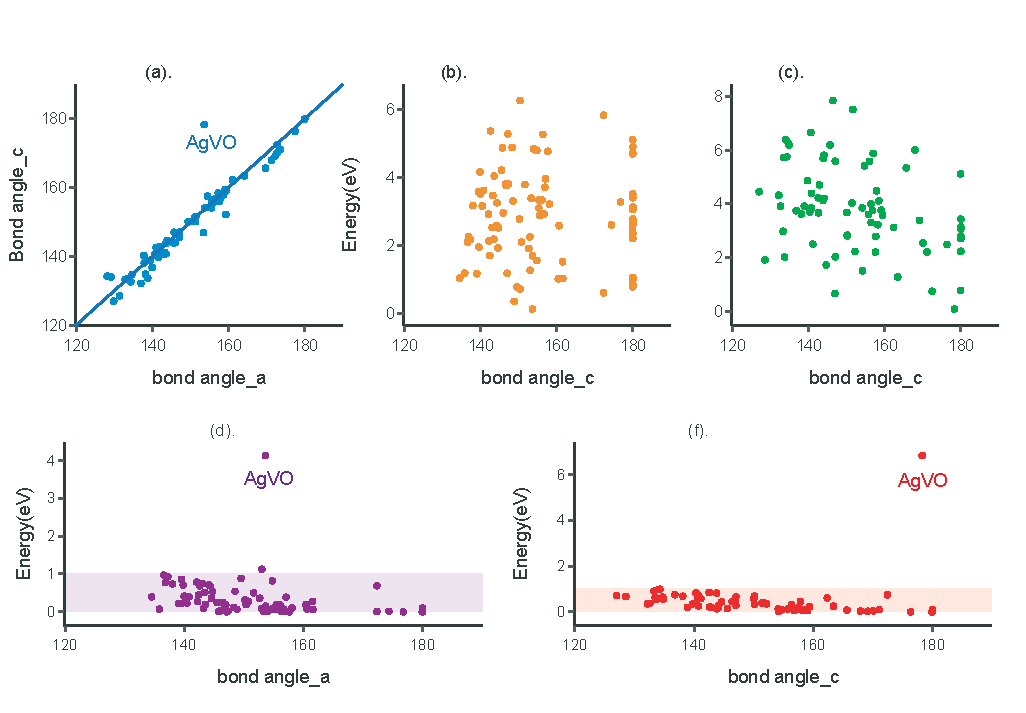
\includegraphics[width=3.2in]{Figures/Fig3.png}
\end{center}
\caption{ The HSE06 functional correction comparing with PBEsol functional for the band gap (orangle), VBM offset(green) and CBM offset(blue) for (a) cubic structure, (b) tetragonal structure, (c) orthorhombic structure. 
}
\label{fig3}
\end{figure}
When a chemometric model is constructed, feature selection is an important step. The goal is to remove (or minimize) the influence of noisy or irrelevant variables that degrade model quality in terms of its performance for the classification problem, so that the final model is thereby built primarily upon variables having high information content.36 Model quality can be evaluated through statistical measures such as sensitivity
(proportion of true positives), specificity (proportion of true
negatives), and accuracy (proportion of true results). Feature
selection is commonly achieved through inspection of Fisher
(F-ratio) scores, the ratio of between-group variability
(explained variance) to within-group variability (unexplained
variance);16 selectivity (S-ratio) scores, which evaluate the
usefulness of each variable in a regression model;37 or loadings
and variable importance in projection (VIP) scores38 (or similar
statistics) during model optimization. Generally, variables with
higher scores contribute more information to the model

Here, we revisit the longstanding problem of predicting the
structures of binary AB compounds, with several goals. First, we
use the CR-FS algorithm applied in PCA space to determine
what combinations of variables (atomic and physical properties) best optimize the discrimination of structure types and
thereby evaluate the reliability of previous structure maps and
gain insight on factors influencing structural preference.
Second, variables retained after feature selection were used to
build PLS-DA and SVM models, with the superior one chosen
to predict the structure of a new compound. Third, we confirm
the existence of a heretofore unknown AB compound through
experiment. Although more than half of the possible AB
compounds (out of all combinations of elements) remain
uninvestigated,


The machine learning models helps us in gaining a fundamental understanding of the most relevant factors of the elements, such as atomic orbital energies, interatomic distances, etc, in the determination of band gaps. We believe that this type of crude estimations of properties can be interesting supplement to standard features.  This crude estimation of properties consists of the calculation of a target property (the experiment band gap) utilizing crude estimators (the calculated PBEsol band gap). This machine learning algorithm no longer needs to predict a target property but rather an correction or a difference between properties calculated with two well-defined methodologies. 



\section{Summary}

In summary, this contribution presents a supervised machine-learning scheme trained using 100 DFT calculated band gaps. Our results show that this method, using a descriptor set based on only composition information, is capable of determination HSE06 functional band gaps, valence band maximum (VBM) and conduction band minimum (CBM) offset with PBEsol functional. 
These results are significant because they present an model that can reliably predict the band gap at a drastically reduced computational cost compared with higher levels of theory.
While this method does not directly correct the PBE band gap for the self-interaction term, it is a powerful way to map computationally cheap methods such as PBEsol to relatively expensive methods such as HSE through finding out the band correction on a specific family compounds. Expansion of this work to other family compounds could enable NNs to augment traditional DFT methods to both lower computational costs and increase accuracy. 
Finally, the success of this method enables us to employ our model to estimate the band gap of other compounds 

\section{Data availability}

The datasets generated during and/or analysed during the current study are available in
the GitHub repository https://github.com/ as well as the
Dryad Digital Repository (doi: 10.5061/). A web application that estimates Eg 

\section{Acknowledgments}

This work was supported by the National Science Foundation Faculty Early Career Development Program DMR-1652994. This research was also supported by the the eXtreme Science and Engineering Discovery Environment (XSEDE) facility, National Science Foundation grant number ACI-1053575, and the Information Technologies (IT) resources at the University of Delaware, specifically the high performance computing resources.

\bibliography{BIB}

\end{document}

% \begin{figure*}[ht!]
% \begin{center}
% 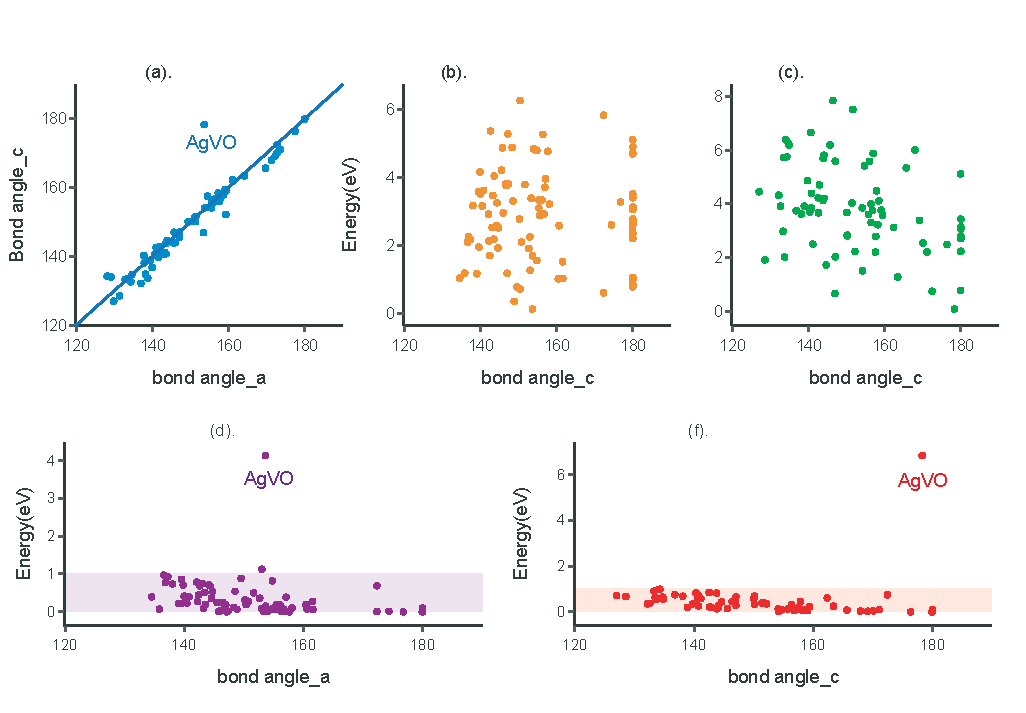
\includegraphics[width=6.0in]{Figures/Fig3.eps}
% \end{center}
% \caption{ (a) the correlation functional relationship between the equatorial and apical bond angle in the orthorhombic structure (space group $Pnma$).
% (b) The DFT band gap of the tetragonal structure (space group $I4_mmm$) as a function of the apical B-O-B bond angles. 
% (c) Two-dimensional map of the DFT band gap of the orthorhombic structure as a function of the apical B-O-B bond angles. 
% (e) The map of the DFT band gap difference between cubic structure and tetragonal structure. 
% (e) The map of the DFT band gap difference between cubic structure and orthorhombic structure. 
% }
% \label{fig4}
% \end{figure*}

% Fig 3. (a) is the map between the apical bond angle and equatorial bond angle in the $Pnma$ structure. It shows a linear function with apical bond angle $\approx$ equatorial bond angle, which is a correction() for the ref\cite{} investigation. 

% Based on our Fig 3.(b) and (c), there is no specific correlation between the DFT band gap and the B-O-B bond angle in the structure. We shows singnificant scatter data dispersion at all the range of the B-O-B bond angle when we change the AB combination. 

% One interesting comparison is the band gap relationship between the cubic (pm$3_bar$m) structure and tetragonal($I4mmm$)\& orthombhedral$pnma$ structure. With octahedral rotation, the band gap not surprisingly increase but always less than 1 eV as shown in Fig3 (d) and (e).